% !TEX encoding = UTF-8 Unicode
%%%%%%%%%%%%%%%%%%%%%%%%%%%%%%%%%%%%%%%%%
% Beamer Presentation
% LaTeX Template
% Version 1.0 (10/11/12)
%
% This template has been downloaded from:
% http://www.LaTeXTemplates.com
%
% License:
% CC BY-NC-SA 3.0 (http://creativecommons.org/licenses/by-nc-sa/3.0/)
%
%%%%%%%%%%%%%%%%%%%%%%%%%%%%%%%%%%%%%%%%%

%----------------------------------------------------------------------------------------
%	PACKAGES AND THEMES
%----------------------------------------------------------------------------------------

\documentclass{beamer}

\mode<presentation> {

% The Beamer class comes with a number of default slide themes
% which change the colors and layouts of slides. Below this is a list
% of all the themes, uncomment each in turn to see what they look like.

%\usetheme{default}
%\usetheme{AnnArbor}
%\usetheme{Antibes}
%\usetheme{Bergen}
%\usetheme{Berkeley}
%\usetheme{Berlin}
%\usetheme{Boadilla}
%\usetheme{CambridgeUS}
%\usetheme{Copenhagen}
%\usetheme{Darmstadt}
%\usetheme{Dresden}
%\usetheme{Frankfurt}
%\usetheme{Goettingen}
%\usetheme{Hannover}
%\usetheme{Ilmenau}
%\usetheme{JuanLesPins}
%\usetheme{Luebeck}
\usetheme{Madrid}
%\usetheme{Malmoe}
%\usetheme{Marburg}
%\usetheme{Montpellier}
%\usetheme{PaloAlto}
%\usetheme{Pittsburgh}
%\usetheme{Rochester}
%\usetheme{Singapore}
%\usetheme{Szeged}
%\usetheme{Warsaw}

% As well as themes, the Beamer class has a number of color themes
% for any slide theme. Uncomment each of these in turn to see how it
% changes the colors of your current slide theme.

%\usecolortheme{albatross}
%\usecolortheme{beaver}
%\usecolortheme{beetle}
%\usecolortheme{crane}
%\usecolortheme{dolphin}
%\usecolortheme{dove}
%\usecolortheme{fly}
%\usecolortheme{lily}
%\usecolortheme{orchid}
%\usecolortheme{rose}
%\usecolortheme{seagull}
%\usecolortheme{seahorse}
%\usecolortheme{whale}
%\usecolortheme{wolverine}

%\setbeamertemplate{footline} % To remove the footer line in all slides uncomment this line
%\setbeamertemplate{footline}[page number] % To replace the footer line in all slides with a simple slide count uncomment this line

%\setbeamertemplate{navigation symbols}{} % To remove the navigation symbols from the bottom of all slides uncomment this line
}

\usepackage{graphicx} % Allows including images
\usepackage{booktabs} % Allows the use of \toprule, \midrule and \bottomrule in tables
\usepackage{xeCJK}
\usepackage{color}
\usepackage{listings}
\usepackage{tikz}
\usepackage{multirow}
\lstset{numbers=left,xleftmargin=10pt,xrightmargin=10pt}

%----------------------------------------------------------------------------------------
%	TITLE PAGE
%----------------------------------------------------------------------------------------

\title[mvc]{MVC Servlet JavaBean} % The short title appears at the bottom of every slide, the full title is only on the title page

\author{张海宁} % Your name
\institute[gzu] % Your institution as it will appear on the bottom of every slide, may be shorthand to save space
{
贵州大学 \\ % Your institution for the title page
\medskip
\textit{hnzhang1@gzu.edu.cn} % Your email address
}
\date{\today} % Date, can be changed to a custom date

\begin{document}

\begin{frame}
\titlepage % Print the title page as the first slide
\end{frame}

\begin{frame}
\frametitle{Overview} % Table of contents slide, comment this block out to remove it
\tableofcontents % Throughout your presentation, if you choose to use \section{} and \subsection{} commands, these will automatically be printed on this slide as an overview of your presentation
\end{frame}

%----------------------------------------------------------------------------------------
%	PRESENTATION SLIDES
%----------------------------------------------------------------------------------------

%------------------------------------------------
\section{MVC} % Sections can be created in order to organize your presentation into discrete blocks, all sections and subsections are automatically printed in the table of contents as an overview of the talk
%------------------------------------------------
\begin{frame}
\Huge{\centerline{MVC}}
\end{frame}
\begin{frame}
\frametitle{什么是MVC}
MVC代表\textcolor{red}{M}odel-\textcolor{red}{V}iew-\textcolor{red}{C}ontroller(模型-视图-控制器)模式。这种模式应用于应用程序(包括但不限于web)的分层开发。

在web开发中,这种模型将web应用分成了三个部分:
\begin{itemize}
\item
\textcolor{red}{M}odel

web应用核心功能
\begin{enumerate}
\item
业务逻辑(\textcolor{red}{Java Bean})
\item
数据库操作(\textcolor{red}{JDBC})
\end{enumerate}

\item
\textcolor{red}{V}iew

主要指与用户的交互界面,通过\textcolor{red}{jsp或html}来构建,负责接收用户输入并转交给控制器。
\item
\textcolor{red}{C}ontroller

负责接收用户的请求,并转发到模型去处理。(\textcolor{red}{servlet})
\end{itemize}

\end{frame}
\begin{frame}
\frametitle{MVC模型}
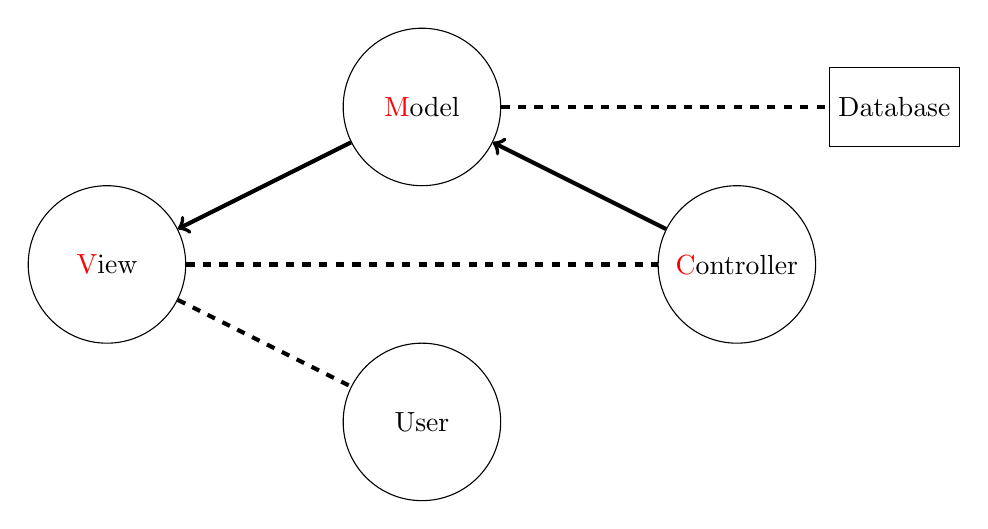
\begin{tikzpicture}
\node (DB) at (10,8) [rectangle,draw,minimum height=10mm] {Database};
\node (M) at (4,8) [circle,draw,minimum size =20mm] {\textcolor{red}{M}odel};
\node (V) at (0,6) [circle,draw,minimum size =20mm] {\textcolor{red}{V}iew};
\node (C) at (8,6) [circle,draw,minimum size =20mm] {\textcolor{red}{C}ontroller};
\node (U) at (4,4) [circle,draw,minimum size =20mm] {User};
\draw [dashed,line width=1.5pt] (M) -- (DB);

\draw [->,line width=1.5pt] (C) -- (M);
\draw [->,line width=1.5pt] (M)-- (V);
\draw [dashed,line width=1.5pt] (V) -- (U);
\draw [dashed,line width=1.5pt] (V) -- (C);
\end{tikzpicture}
\end{frame}
\begin{frame}
\frametitle{MVC的具体实现}
在不引入框架的情况下:

\begin{table}
\begin{tabular}{cc}
\toprule
\textbf{M/V/C} & \textbf{technology}\\
\midrule
V & jsp,html\\
C & servlet\\
M & java bean\\
\bottomrule
\end{tabular}
\caption{MVC的无框架实现}

\end{table}
\end{frame}
\section{servlet}
\begin{frame}
\Huge{\centerline{servlet}}
\end{frame}
\begin{frame}
\frametitle{什么是servlet}
servlet是\textcolor{red}{运行在web服务器端的java程序}。
\begin{enumerate}
\item
\textcolor{red}{封装了对HTTP请求}的处理
\item
运行\textcolor{red}{需要servlet容器}支持(比如tomcat、weblogic等)。
\end{enumerate}


servlet先于jsp产生,但是其代码组织形式是\textcolor{red}{将html代码混杂在java代码中},给web程序设计带来了很多不便,比如负责网页设计的\textcolor{red}{美工人员也需要学习java知识},才能进行页面的设计,在程序设计中,servlet产生的动态网页又需要在代码中\textcolor{red}{编写大量输出html标签的语句}。

基于以上原因,Sun公司提出了jsp技术。jsp是一种在servlet规范之上的动态网页技术,jsp文件在第一次被请求时,会被编译成servlet文件,再通过容器调用servlet进行处理。

\end{frame}
\begin{frame}
\frametitle{为什么使用servlet}
由于以下两个特点,
\begin{enumerate}
\item
servlet由java语言编写,因此其可获得java语言的所有功能支持
\item
servlet对web应用进行了封装,可对http请求进行相应的处理
\end{enumerate}
再加上\textcolor{red}{jsp}承担了原来servlet中的\textcolor{red}{负责页面显示}的部分,因此现在的\textcolor{red}{servlet}就比较适合用来\textcolor{red}{处理web系统的业务逻辑}。
\end{frame}
\begin{frame}[fragile]
\frametitle{servlet代码片断}
\begin{lstlisting}
 while(enu.hasMoreElements()){
 String attr = enu.nextElement();
  if(attr.equals("user")){
    user = (String)session.getAttribute("user");
    out.print("你好,"+user+"。");
    out.print("<form action=\"logout.jsp\"
        method=\"post\">");
    out.print("<input type=\"submit\" 
        value=\"logout\"></form>");
    break;
  }
}
\end{lstlisting}
\end{frame}
\begin{frame}[fragile]
\frametitle{servlet代码结构}

 在eclipse中,右键点击项目,选择新建,servlet,即可建立一个servlet.
\begin{lstlisting}
@WebServlet("/Reg")
public class Reg extends HttpServlet {
private static final long serialVersionUID = 1L;    
  public Reg() {
        super();
    }
 protected void doGet(HttpServletRequest req, 
     HttpServletResponse resp) 
     throws ServletException, IOException {
 }
  protected void doPost(HttpServletRequest req, 
     HttpServletResponse resp) 
     throws ServletException, IOException {
  }
}
\end{lstlisting}
\end{frame}

\begin{frame}
\frametitle{servlet使用示例}
以注册为例,展示servlet的使用方法。
原来的注册功能是通过teacher\_add.jsp页面来实现的。

接下来将采用Reg这个servlet来实现相同的功能,主要步骤为:

\begin{enumerate}
\item
更改form的action地址为Reg这个servlet
\item
完善Reg这个servlet里的doPost()方法,以处理表单通过post提交过来的数据
\end{enumerate}
\end{frame}
\begin{frame}[fragile]
\frametitle{更改form的action}
\begin{lstlisting}
<form action="Reg" method="post">
\end{lstlisting}
\end{frame}
\begin{frame}[fragile]
\frametitle{完成Reg里的doPost()方法}
\begin{lstlisting}
protected void doPost(... , ...)... {
// 设置request传递过来值的编码,并获取传递值
request.setCharacterEncoding("utf-8");
String id = request.getParameter("staffid");
String name = request.getParameter("nm");
//get current date and time
LabDate ld = new LabDate();  
String time = ld.getDtTm();
//write to database
String[] fields= {"id","name","logDate"};
String[] values= new String[3];
values[0]=id; values[1]=name; values[2]=time;
Db db = new Db();
int i = db.writeDb("teachers", fields, values);
db.getClose();
}
\end{lstlisting}
\end{frame}
\begin{frame}[fragile]
\frametitle{完成Reg里的doPost()方法-II}
\begin{lstlisting}
protected void doPost(... , ...)... {
// 设置request传递过来值的编码,并获取传递值
//get current date and time
//write to database
int i = db.writeDb("teachers", fields, values);
db.getClose();
String rz="";
if(i==1) {
  rz = "Done! Will return  in 3 seconds.";
}else {
  rz = "Sth wrong! Will return  in 3 seconds.";
}
response.getWriter().print(rz);
response.setHeader("refresh","3,URL=teacher.jsp");
}
\end{lstlisting}
\end{frame}

\begin{frame}{servlet过滤器}
先观察下图:
\begin{figure}
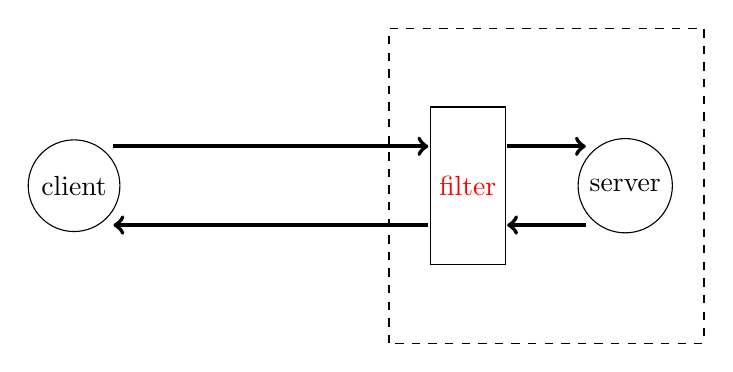
\begin{tikzpicture}
\node (c) at (1,5) [circle,draw] {client};

\node (f) at (6,5) [rectangle,draw,minimum height=20mm] {\textcolor{red}{filter}};
\node (s) at (8,5) [circle,draw] {server};
\draw [dashed,label=above:webserver] (5,3) rectangle (9,7) ;
\draw [->,line width=1.5pt] (1.5,5.5) -- (5.5,5.5); 
\draw [<-,line width=1.5pt] (1.5,4.5) -- (5.5,4.5); 
\draw [->,line width=1.5pt] (6.5,5.5) -- (7.5,5.5); 
\draw [<-,line width=1.5pt] (6.5,4.5) -- (7.5,4.5); 

\end{tikzpicture}
\caption{the position and function of a filter}
\end{figure}
可以看出,filter是介于client和server端的一个“关卡”,其负责“过滤”信息流(这个过滤器可以有多个,形成过滤器链)。
\end{frame}
\begin{frame}[fragile]{创建一个filter}
创建一个filter,禁止特定id的用户注册(\textcolor{red}{chain.doFilter()})。

创建过程与创建servlet类似。

FilterReg.java的主要代码如下所示:
\begin{lstlisting}
@WebFilter(filterName = "/FilterReg",
      urlPatterns = "/Reg")
public class FilterReg implements Filter {
  public void doFilter(ServletRequest request, 
  ServletResponse response, FilterChain chain)  {
  HttpServletRequest req = 
      (HttpServletRequest) request; 
  String id = request.getParameter("staffid");
  System.out.println("staffid is: "+id);
  // pass the request along the filter chain
  chain.doFilter(request, response);
  }
}
\end{lstlisting}
\end{frame}
\begin{frame}[fragile]{chain.doFilter()}
Pay attention to 
\textcolor{red}{chain.doFilter()}.
\begin{lstlisting}
public void doFilter(ServletRequest request, 
    ServletResponse response, FilterChain chain){
HttpServletRequest req = 
  (HttpServletRequest) request; 
String id = request.getParameter("staffid");
System.out.println("staffid is: "+id);
	
// pass the request along the filter chain
chain.doFilter(request, response);
		
HttpServletResponse resp = 
    (HttpServletResponse) response;
resp.getWriter().print("add is done. Stay here.");
//resp.setHeader("refresh", "3,URL=index.jsp");
}
\end{lstlisting}
\end{frame}

\begin{frame}{监听器}
\textcolor{red}{监听}是对\textcolor{red}{特定事件}进行关注。

所谓监听器就是对特定事件的发生做出反应,比如你点击了什么按钮等等。
\begin{table}
\begin{tabular}{ll}
\toprule
\textbf{Listener接口}&\textbf{Event类}\\
\midrule
ServletContextListener&ServletContextEvent\\
ServletContexAttributeListener&ServletContextAttributeEvent\\
HttpSessionListener&\multirow{2}{*}{HttpSeesionEvent}\\
HttpSessionActivationListener&\\
HttpSessionAttributeListener&\multirow{2}{*}{HttpSessionBindingEvent}\\
HttpSessionBindingListener&\\
ServletRequestListener&ServletRequestEvent\\
ServletRequestAttributeListener&ServletRequestAttributeEvent\\
\bottomrule
\end{tabular}
\caption{Listener接口与Event类}
\end{table}
\end{frame}


\begin{frame}[fragile]{使用servlet处理文件上传I}
form的主要代码为(class\_apply.jsp):
\begin{lstlisting}
<form action="ServletClassArrange" 
  enctype="multipart/form-data" method="post">
<table>
<tr><td>
上传实验指导书:<input type="file" name="guideBook" >
   </td></tr>
<tr><td>
<button type="submit">submit</button>
   </td></tr>
</table>
</form>
\end{lstlisting}
\end{frame}
\begin{frame}[fragile]{使用servlet处理文件上传II}
Servlet的主要代码为(ServletClassArrange.java):
\begin{lstlisting}
@WebServlet("/ServletClassArrange")
@MultipartConfig
public class ServletClassArrange 
   extends HttpServlet {
 protected void doPost(......){
  request.setCharacterEncoding("utf-8");
  Part pt = request.getPart("guideBook");
  String fName = pt.getSubmittedFileName();
  System.out.println("the file is:"+fName);
  System.out.println(
   this.getServletContext().getRealPath("/")+fName);
  pt.write("/Users/hainingzhang/Downloads/"+fName);
  System.out.println("success uploaded!");
 }
}
\end{lstlisting}
\end{frame}
%---------------------------------------------
\section{javabean}
\begin{frame}
\Huge{\centerline{javabean}}
\end{frame}
\begin{frame}{什么是javabean}
如果一个类满足以下条件:
\begin{enumerate}
\item
All properties private (use getters/setters)
\item
A public no-argument constructor
\item
Implements Serializable
\end{enumerate}
则就称这个类是一个javabean。
\end{frame}
\begin{frame}[fragile]{serializable}
如果想将一个java对象保存到文件中,那么这个对象必须是可序列化的(serializable),也就是说这个对象的类需要是可序列化的。
\begin{block}{Teacher类实现序列化}
\begin{lstlisting}
import java.io.Serializable;

public class Teacher implements Serializable{
   private static final long serialVersionUID = 1L;
}
\end{lstlisting}
\end{block}
\end{frame}
\begin{frame}{为什么要使用javabean}
使用javabean可以使html代码和java代码尽可能的分离,将java代码单独封装成为一个处理某种业务逻辑的类,然后在jsp页面中调用此类。以\textcolor{red}{简化jsp页面和提高java程序代码的重用性}。
\end{frame}
\begin{frame}[fragile]{Teacher}
定义Teacher类,该类为封装教师对象的javabean。
\begin{lstlisting}
//Teacher.java
package bean;
import java.io.Serializable;
public class Teacher implements Serializable{
 private static final long serialVersionUID = 1L;
 private String staffid,nm,logDate;	
 public Teacher() {}
 public void setstaffid(String id){this.staffid=id;}
 public void setnm(String name) {this.nm=name;}
 public void setlogDate(String logDate) {
   this.logDate=logDate;}
 public String getstaffid() { return staffid; }
 public String getnm() { return nm;  }
 public String getlogDate() { return logDate;  }
}
\end{lstlisting}

\end{frame}
\begin{frame}[fragile]{与javabean相关的几个jsp标签}
\begin{enumerate}
\item
jsp:useBean

实例化一个对象
\item
jsp:setProperty

为一个属性赋值
\item
jsp:getProperty

获取一个属性值
\end{enumerate}
\begin{lstlisting}
//teacher_add.jsp
<jsp:useBean id="teacher" class="bean.Teacher">
 </jsp:useBean>
<jsp:setProperty name="teacher" property="nm"
 value="贵州大学" />
<jsp:getProperty property="nm" name="teacher"/>

\end{lstlisting}

\end{frame}

\begin{frame}[fragile]{对javabean属性赋值与获取javabean属性}
在jsp页面中,对javabean属性赋值与获取javabean属性。
\begin{lstlisting}
//teacher_add.jsp
<% request.setCharacterEncoding("utf-8"); %>
<jsp:useBean id="teacher" class="bean.Teacher">
 </jsp:useBean>
<jsp:setProperty name="teacher" property="*" />
<table>  <tr> <th>staffid</th> <th>nm</th> 
      <th>logDate</th> </tr>  <tr> <td>
<jsp:getProperty property="staffid" name="teacher"/>
</td><td>
<jsp:getProperty property="nm" name="teacher"/>
</td><td>
<jsp:getProperty property="logDate" name="teacher"/>
</td></tr></table>
\end{lstlisting}

\end{frame}

\begin{frame}{作业}
\begin{enumerate}
\item
使用session记录登陆状态
\item
练习servlet和javabean的使用
\item
学习jsp+servlet+javabean联合使用

\url{https://github.com/danielniko/SimpleJspServletDB}
\end{enumerate}
\end{frame}
%------------------------------------------------

\begin{frame}
\Huge{\centerline{The End}}
\end{frame}

%---------------------------------------
\section{Appendix}

\begin{frame}
\Huge{\centerline{Appendix}}
\end{frame}
\begin{frame}{Appendix}
\begin{block}{ppt、项目源代码及实验指导书的地址}
\begin{enumerate}
\item
ppt

\url{https://github.com/gmsft/ppt/tree/master/javaweb}
\item
lab-java项目

\url{https://github.com/gmsft/javaweb}

\item
实验指导书

暂无,拟放在ppt的仓库里
\end{enumerate}
\end{block}
\end{frame}

\begin{frame}{ServletRequest和HttpServletRequest}
public interface HttpServletRequest\\
extends ServletRequest\\
Extends the ServletRequest interface to provide request information for HTTP servlets.
\end{frame}

%----------------------------------------------------------------------------------------

\end{document} 